\documentclass{article}

\usepackage[a4paper]{geometry}
\usepackage[ngerman]{babel}
\usepackage[utf8]{inputenc}
\usepackage[T1]{fontenc}
\usepackage{graphicx}
\usepackage{fancyhdr}
\usepackage{amsmath}
\usepackage{xcolor}
\usepackage{float}
\usepackage{hyperref}

\graphicspath{{./images/}}

\pagestyle{fancyplain}
\fancyhf{}
\lhead{\fancyplain{}{Mara Schulke} }
\rhead{\fancyplain{}{\today}}
\cfoot{\fancyplain{}{\thepage}}

\newcommand{\annotation}[1]{
    \begin{quote}
    	\begin{textit}{#1}\end{textit}
    \end{quote}
}

\newcommand{\figuresource}[1]{
	\begin{center}Quelle: {#1}\end{center}
}

\renewcommand*{\thesection}{Kapitel \arabic{section}}
\renewcommand*{\thesubsection}{\alph{subsection})}
\renewcommand*{\thesubsubsection}{\arabic{subsubsection})}

\begin{document}

\begin{titlepage}
	\begin{center}
		\begin{Large}
			Technische Hochschule Brandenburg \\[1em]
		\end{Large}
		
		IT Sicherheit \\
		Informatik und Medien \\
		Biometrie – Dr.\ Tobias Scheidat
	\end{center}
	
	\vfill

	\begin{center}
		\Large{Übungsaufgaben}\\[0.5em]
		\large{Wintersemester 2024}\\[0.25em]
		\large{Abgabetermin \today}
	\end{center}

	\vfill

	\begin{center}
		Mara Schulke \\ Matr-Nr. 20215853
	\end{center}
\end{titlepage}


\tableofcontents

\listoffigures

\newpage

\section{}

\subsection{Erl\"autern Sie den Begriff Benutzerauthentifizierung}

Benutzerauthentifizierung beschreibt den formalen Prozess der Verifikation der Nutzeridentität innerhalb 
eines Systems. Dies kann anhand einer der drei Authentifizierungsschemata stattfinden: Wissen, Besitz oder 
Biometrie.

\subsection{Definieren Sie den Begriff biometrische (Benutzer-)Erkennung}
\annotation{Grenzen Sie zu der vorherigen Aufgabe ab.}
Die biometrische Benutzer-Erkennung ist streng genommen ein Teilbereich der Benutzerauthentifizierung. Wie 
oben genannt lässt sich die Benutzerauthentifizierung mittels Wissen, Besitz oder Biometrie durchführen.

Im Gegensatz zu den Schemata Wissen und Besitz fokussiert sich die biometrie-gestützte Erkennung/
Authentifizierung nicht auf Nachweismöglichkeiten die extrinsisch mit einem Individuum verknüpft sind 
(Passwort, Schlüssel, ..) sondern auf intrinsische Nachweismöglichkeiten wie die Physiologie oder das
Verhalten eines Individuums.

Außerhalb der Authentifizierung befasst sich die biometrische Erkennung mit der statistischen Zuordnung 
von Eingabedaten zu einem hinterlegten biometrischen Fingerprint. Dies umfasst z.B. die Auswertung von 
Sprachaufnahmen um regionale Sprachmuster zu erkennen.

\subsection{Erläutern Sie die 11 Merkmale der Bertillonage}
\annotation{{\"U}berlegen Sie: wie konnte mit den damaligen Mitteln eine Identifikation durchgeführt werden?}

Die 11 Merkmale mit denen damals die Bertillonage durchgeführt wurde lauten: Körpergröße, Spannweite der 
Arme, Sitzhöhe, Kopflänge, Kopfbreite, Länge und Breite des rechten Ohrs, Länge des linken Fußes sowie 
Längen des linken Mittelfingers, des linken kleinen Fingers und des linken Unterarms (Auszug aus dem 
Skript 1.4).

Die Vorgehensweise der Bertillonage ist der der in der DNA-basierten Identifikation recht ähnlich (zumindest 
oberflächlich). In beiden Fällen werden bestimmte Merkmale eines Individuums extrahiert (ie. Marker).
Je mehr Marker zwischen zwei Datensätzen übereinstimmen, desto wahrscheinlicher ist es, dass es sich um 
das gleiche Individuum handelt. Der Abgleich eines einzelnen Individuums ist nicht rechenaufwendig, daher 
war dieses Verfahren bereits im 19. Jahrhundert möglich.

\subsection{Was sind biometrische Charakteristika und welche zwei grundsätzlichen Kategorien gibt es hier?}
\annotation{Klassifizieren Sie biometrische Merkmale in die zwei grundsätzlichen Kategorien und benennen Sie jeweils mindestens vier Beispiele für jede?}	

Es gibt die grundsätzliche Unterteilung zwischen Online- und Offline- Merkmalen. Diese unterscheiden sich
primär hinsichtlich ihres Aufzeichnungszeitpunktes: Online Merkmale können nur während einer Handlung 
aufgenommen werden (z.B. während eine Notiz geschrieben wird) wohingegen Offline-Daten auch im Nachhinein
verfügbar sind (z.B. der beschriebene Notizzettel).

Beispiele für Online-Merkmale sind z.B. Sprachaufnahmen, ein Video von einer handschriftlichen Notiz, das 
Tippverhalten an dem Computer, eine Aufnahme vom Geh-Verhalten. Beispiele für Offline-Merkmale sind z.B. 
Fußstapfen, ein Foto von einer handschriftlichen Notiz, Fingerabdrücke und Körpermaße.

\subsection{Erklären Sie: was verstehen wir unter dem Begriff Lebenderkennung?}

Die Lebenderkennung fokussiert sich primär auf verhaltensbasierte Merkmale, da diese im Gegensatz zu
physiologischen Merkmalen inhärent nur von lebenden Subjekten entnehmen lassen. Diese Merkmale bieten 
somit eine (weitgehende) Sicherheit gegen Spoofing-Attacken.

\newpage

\section{}

\subsection{Finden und beschreiben Sie für jeden der 6 Sicherheitsaspekte ein Beispiel, wie diese speziell für biometrische Systeme relevant sein k\"onnen!
}

\subsubsection*{Vertraulichkeit}

Ein biometrisches System, das für die Authentifizierung eingesetzt wird, sollte ähnliche 
Sicherheitscharakteristika haben wie eine passwortbasierte Authentifizierung. D. h. es sollte vergleichbar
schwer für einen Angreifer sein, ein biometrisches Authentifizierungsverfahren zu umgehen, wie für  
herkömmliche, da sonst die Vertraulichkeit der Daten durch den Einsatz des biometrischen Systems
gefährdet ist.

\subsubsection*{Integrität}

Die Verifikationsdaten eines biometrischen Systems sollten sich ausschließlich nach der 
Sicherstellung der Identität des Benutzers ändern lassen. Idealerweise mittels 
Multifaktorauthentifizierung.

\subsubsection*{Verfügbarkeit}

Um die Verfügbarkeit eines Systems nicht durch den Einsatz von Biometrie gefährden sollte das biometrische 
System ausgiebige Tests im Hinblick auf dessen Zuverlässigkeit bestehen. Wenn das Gesamtsystem nicht mehr
nutzbar ist, da das biometrische Authentifizierungssystem versagt, wird die allgemeine Verfügbarkeit 
beeinträchtigt.

\subsubsection*{Authentizität}

Die Verifikationsdaten eines biometrischen Systems sollten idealerweise mit einem, bereits bekannten, dem 
Individuum zugeordneten Schlüsselpaar signiert werden um diese zweifelsfrei an die Identität des Nutzers 
zu binden.

\subsubsection*{Verbindlichkeit}

Alle Änderungen an den hinterlegten Verifikationsdaten, sowie jegliche Authentifizierungsvorgänge bzw. 
Versuche sollten dokumentiert werden, damit die Authentifizierung eines Nutzers zurückverfolgt werden 
kann.

\subsubsection*{Privatsphäre}

Ein biometrisches System sollte niemals rohe biometrische Daten über ein Individuum speichern, vielmehr 
sollte es entweder eine verschlüsselte Version speichern oder idealerweise einen Fingerprint, der sich aus 
den Eingabedaten konstruieren lässt, sich aber nicht ohne weiteres zurück in eindeutige biometrische 
Eigenschaften übersetzen lässt.

\subsection{Geben Sie 3 Beispiele (mit einer kurzen Erläuterung), was bei Security-by-Design für biometrische Systeme berücksichtigt werden sollte!}

\subsubsection*{Nicht-Zurückverfolgbarkeit}

Aus einem biometrischen System sollten nie genug Daten gewonnen werden können, um den Nutzer eindeutig zu 
identifizieren (ohne das system Selbst zu Verwenden). Ie. es sollten keine Rückschlüsse auf physische 
Eigenschaften (Hautfarbe, Größe, Geschlecht, etc.) aus den im System hinterlegten Daten möglich sein.

\subsubsection*{Need-to-know}

Lediglich biometrische Merkmale aufzeichnen, die einen konkreten Verwendungszweck für die Aufgabe des 
biometrischen Systems haben. Mehr Daten aufzuzeichnen als notwendig birgt das Risiko der Zweckentfremdung.

\subsubsection*{Geringe False-Accept-Rate}

Gerade so viele biometrische Merkmale sammeln, dass die Fehlerquote des biometrischen Systems für falsche 
Authentifizierungen vernachlässigbar gering ausfällt. 

\subsection{Geben Sie 3 Beispiele mit einer kurzen Erläuterung, was bei Ethik-by-Design für biometrische Systeme berücksichtigt werden sollte!}

\subsubsection*{Randomisierte Tests}

Ein biometrisches System sollte mit heterogenen Nutzern getestet werden um sicherzustellen, dass 
marginalisierte Gruppen nicht benachteiligt werden. Beispielsweise sollte sichergestellt werden, dass eine 
Gesichtserkennung zuverlässig über ethnische Gruppen hinweg funktioniert, anstatt nur mit einer Ethnie zu 
testen.

\subsubsection*{Verhinderung von Zweckentfremdung}

Ein System zur biometrischen Authententifizierung ist in den meisten Fällen wahrscheinlich ethisch 
unbedenklich, wohingegen ein System zur Identifizierung anhand von biometrischen Merkmalen kritisch 
betrachtet werden kann. Daher ist es wichtig, bei der Entwicklung eines biometrischen Systems 
sicherzustellen, dass dieses bzw. die Daten, die das System verarbeitet, nicht entfremdet zur 
Identifikation von Individuen benutzt werden können.

\subsubsection*{Datenhoheit liegt beim Nutzer}

Dem Nutzer muss es freistehen, das System ohne biometrische Authentifizierung zu verwenden damit dieser 
die Datenhoheit behält. Ie. ein Nutzer sollte nicht gezwungen werden seine biometrischen Merkmale 
aufzuzeichnen, ohne dass eine Nutzung der biometrischen Authentifizierung beabsichtigt ist.

\newpage

\section{}

\subsection{Aus welchen Phasen besteht das Prozess-/ Mustererkennungsmodell zur biometrischen Erkennung: benennen \& erklären Sie!}

\begin{figure}[ht]
	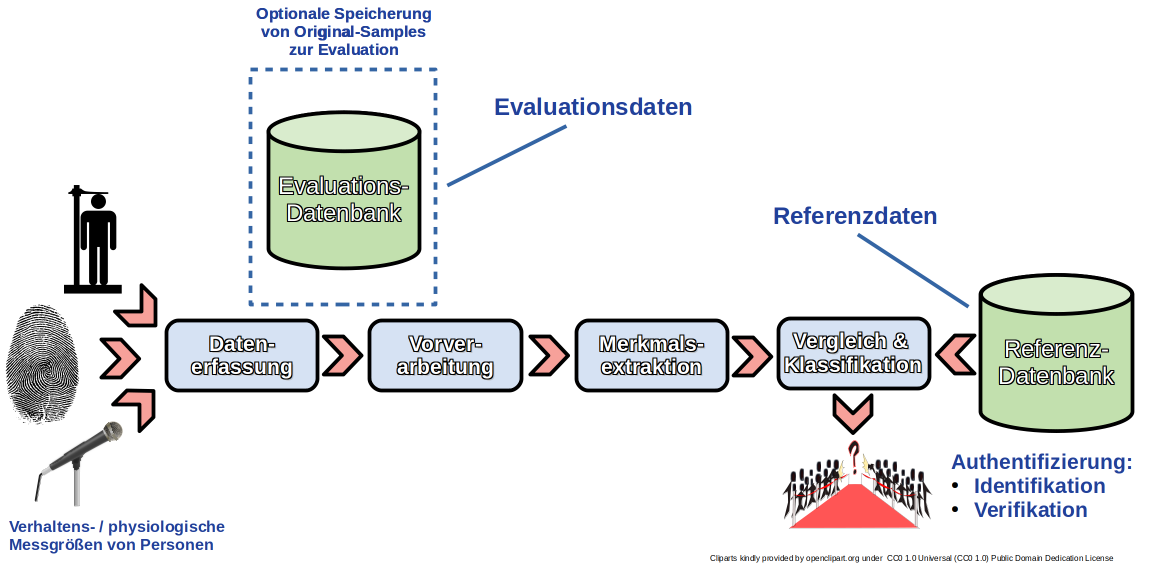
\includegraphics[width=0.5\textwidth]{assets/pipeline-id}
	\centering
	\caption{Biometrie-Pipeline}
	\figuresource{Biometrie Skript}
\end{figure}

Eine einfache biometrische Pipeline zur Erkennung von Mustern / zur Authentifizierung besteht aus den 
folgenden vier Phasen:

\subsubsection*{Datenerfassung}

Die erste Phase des Modells beschäftigt sich mit der Erfassung der Daten aus der physischen Welt mittels 
eines Sensors. Dies kann ein Fingerabdruck-Sensor sein, sowie ein Mikrofon oder eine Kamera.

\subsubsection*{Vorverarbeitung}

Nachfolgend müssen die Rohdaten vor-verarbeitet werden. Dies umfasst die Filterung, Aufbereitung, 
Korrektur oder Konvertierung der aufgezeichneten Daten um eine einfachere Verarbeitung in den folgenden 
Phasen zu ermöglichen.

\subsubsection*{Merkmalsextraktion}

Anschließend müssen aus den vor-verarbeiteten Rohdaten Merkmale bzw. Merkmalsvektoren extrahiert werden um
verschiedene Eingabedaten im gleichen Raum miteinander zu vergleichen. Die Extraktion ermöglicht einen 
sehr effizienten Vergleich, da z.B. im Falle von Kameradaten nicht Bilddaten miteinander abgeglichen 
werden, sondern die Eigenschaften die aus den Bilddaten gewonnen wurden. Somit kann eine Suche in der 
Referenzdatenbank schnell vonstatten gehen.

\subsubsection*{Vergleich \& Klassifikation}

Die letzte Phase der Pipeline ist der Vergleich und die Klassifizierung des Merkmalsvektors aus dem 
vorherigen Schritt mit denen in der Referenzdatenbank. Hier werden die verschiedenen Vektoren mittels 
mathematischer Vergleichsoperationen/modelle korreliert und bei gegebener Nähe wird eine positive 
Entscheidung zurückgegeben.

Die genaue Umsetzung obliegt dem System, so kann jedes System unterschiedliche Schwellwerte für eine 
Entscheidung heranziehen und/oder Entscheidungen aus mehreren verschiedenen Merkmalen kombinieren. 


\subsection{Skizzieren Sie den Prozess des biometrischen Enrollments, wie im Kurs eingeführt!}

Der Prozess des biometrischen Enrollments ist dem der Authentifizierung sehr ähnlich; da lediglich die 
letzte Phase ``Vergleich \& Klassifikation'' entfällt. Nach der dritten Phase (Merkmalsextraktion) wird
der/die Merkmalsvektor(en) in einer Referenzdatenbank hinterlegt gegen die dann die Authentifizierung 
stattfinden kann.


\subsection{Skizzieren Sie den Prozess des biometrischen Authentifikation, wie im Kurs eingeführt!}

Der Prozess der Authentifikation umfasst das \textit{einmalige} abgleichen $n$ Merkmerkmalsvektoren 
gegenüber der, in der Referenzdatenbank hinterlegten Vektoren, für einen Nutzer. 
Die Authentifikation grenzt sich gegenüber der Identifikation dahingehend ab, dass keine Suche innerhalb 
der Referenzdaten stattfindet.

\subsection{Erklären Sie folgende Begriffe}

\subsubsection{Variabilität, Intra-Personen und Inter-Personen Variabilität}

\textbf{Variabilität} im allgemeinen bezieht sich auf die (wie unter Aufgabe \textit{3e)} erklärt) auf
die Bandbreite der Messungen von biometrischen Daten. Es gibt zwei unterschiedliche Bandbreiten die 
normalerweise betrachtet werden:

Die \textbf{Intra-Personen Variablität} bezieht sich auf die Schwankungen der Messungen von biometrischen
Daten der gleichen Person. Beispielsweise unterliegen biometrische Eigenschaften natürlichen Schwankungen,
wie z.B. offensichtlich erklärbar (ie. durch Nahrungszufuhr) bei dem Gewicht einer Person. Allerdings
bezieht sich die Variabilität nicht nur auf die rein physische Schwankung sondern betrachtet auch die
Fehlerraten bei der Messung.

Die \textbf{Inter-Personen Variablität} bezieht sich dementsprechend auf die Schwankungen der Messwerte 
über alle Personen / Benutzer des biometrischen Systems hinweg. Beispielsweise ließe sich hier die 
Gesamtverteilung der Körpergröße über alle Menschen hinweg als \textbf{Inter-Personen Variablität} der 
Körpergröße beschreiben.

\subsubsection{Benennen Sie mindestens drei Ursachen für Variabilität}

Variabilität kann – wie oben genannt – verschiedene Ursachen haben:

\begin{enumerate}
	\item Biologische / Physische Schwankungen – Beispielsweise ändert sich das Gewicht über den Tag hinweg.
	\item Biologische Unterschiede – So unterliegen biometrische Parameter immer dem Einfluss der biologischen Gegebenheiten (z.B. Geschlecht, Ethnie etc.)
	\item Mess-Ungenauigkeit – Leichte Änderungen der Werte über Messungen hinweg können auch einer Ungenauigkeit der Sensorik zugrunde liegen.
\end{enumerate}
 
\subsection{Welche Eigenschaften sind an biometrische Merkmale zu stellen, benennen \& erklären Sie!}
 
\subsubsection*{Variabilität}

Die Variabilität beschreibt die Eigenschaft eines Merkmals über viele Messungen hinweg. Sie kann in den 
Dimensionen Intra-Person und Inter-Klasse betrachtet werden.

Ein gutes biometrisches Merkmal hat die Eigenschaft einer geringen Intra-Personen-Variabilität – also 
einer möglichst konstanten Messbarkeit innerhalb der gleichen Person \textbf{bei gleichzeitiger} möglichst
großer Inter-Class-Variabilität – also einer möglichst breitgestreuten Verteilung des Merkmals innerhalb 
der Klasse an Subjekten.

\subsubsection*{Trennschärfe}

Die Trennschärfe ist eingeführt als möglichst großer Grad zwischen der hohen Intra-Personen-Variabilität 
und Inter-Klassen-Variabilität. Je klarer ein Merkmal zu messen ist und je breit gestreuter die Messungen 
über alle Subjekte hinweg sind, desto Aussagekräftiger ist die Messung über die Identität.

\subsubsection*{Erfassbarkeit}

Die Erfassbarkeit eines Merkmals beschreibt die Betrachtung des realistisch-möglichen Einsatzes des 
Merkmals in einem biometrischen System mit verfügbaren Sensoren. Beispielsweise lassen sich Bild-Daten 
eines Subjektes leicht erfassen wohingegen DNA-Daten sehr aufwändig zu beschaffen sind.

\subsubsection*{Leistung}

Leistung beschreibt den zeitlichen Aspekt der Erfassung bzw. Verarbeitung. D.h. wenn ein Merkmal bspw. 
extreme Mengen an Daten generiert, könnte dies u.U. zu Performance-Problemen im biometrischen System 
führen.

\subsubsection*{Privatsphäre}

Die letzte Eigenschaft von Merkmalen ist dahingehend wichtig, dass bestimmte Datensätze Aussagekräftiger 
über Anwendungszweck-Fremde Daten (wie z.B. Herkunft sind, als andere) und somit a) Vorsicht im Umgang und 
bei der Speicherung mit solchen Merkmalen geboten ist und b) eine ethische Betrachtung stattfinden sollte, 
welche Merkmale für ein biometrisches System verwendet werden.

\newpage

\subsection{Erklären Sie beispielhaft anhand eines Häufigkeitshistogramms die Merkmalsverteilungen „Intra-Class“, „Inter-Class“}


\begin{figure}[ht]
	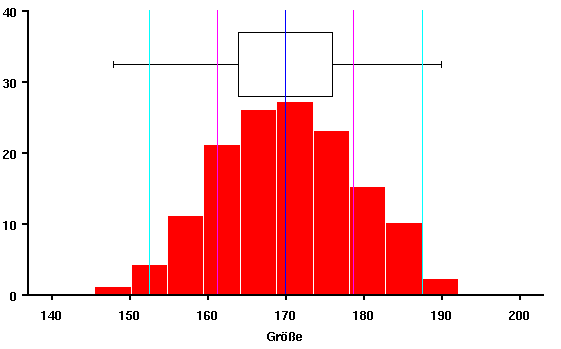
\includegraphics[width=0.5\textwidth]{assets/histogramm}
	\centering
	\caption{Histogramm: Größe}
	\figuresource{Universität Münster 
		(\href{https://campus.uni-muenster.de/fileadmin/einrichtung/ibkf/lehre/skripte/biomathe/bio/eda/help/eda15.html}{campus.uni-münster.de})
	}
\end{figure}

Wie in der Abbildung 2) zu erkennen reichen die Messwerte in der oben angeführten Beispielverteilung
von ca. 145cm bis zu ca. 195cm. Diese Spanne beschreibt die Inter-Class Variabilität von allen Menschen
in der aufgezeichneten Gruppe. Die Intra-Class- (oder Intra-Personen-) Variabilität fällt deutlich 
geringer aus: Die Körpergröße ist vergleichsweise (z.B. im direkten Vergleich mit dem Merkmal Gewicht)
biologisch Stabil (also unterliegt lediglich kleinen Schwankungen) und der größte Anteil hier
dürfte durch Fehlerraten während der Messung entstehen.

\subsection{Überlegen Sie: bislang bezog sich die „Inter-Class“ Verteilung ja nur auf die Merkmale „anderer“ Personen als die der authentischen, mit ihren eigenen Merkmalen. Wie würde sich die Situation für gezielte Fälschungen im Diagramm darstellen, welche Veränderungen können Sie hier vorhersehen? Beschreiben oder skizzieren Sie im Diagramm!}

Dies kommt auf die Abweichung des zu fälschenden Messwertes von dem Medianwert aller Messungen an.
Somit ließe sich ein Angriff relativ eindeutig (und bereits nach wenigen böswilligen 
Authentifizierungsversuchen) erkennen, wenn der gefälschte Messwert mehrere Standardabweichungen vom 
Median entfernt liegt. (Da es somit zu einer verhältnismäßig starken Änderung des Medianwertes käme). 
Visuell wäre ein Angriff daran zu erkennen, wenn sich der Balken (bspw. bei 145cm) innerhalb von kurzer 
Zeit, stark erhöht und somit eine signifikante Auswirkung auf die berechnete Standardabweichung hätte. Bei 
einer großen Menge (im Verhältnis zu den gesamten Messdaten) an Fälschungen einer Messung nahe am 
Medianwert würde der mittlere Balken (über der blauen Linie) drastisch Ansteigen. Ebenfalls hier wäre
dies durch die Beobachtung der Standardabweichung zu erkennen.

\newpage

\section{}

\subsection{Definieren Sie die folgenden biometrischen Fehlerraten}

\subsubsection{False Non-Match Rate (FNMR)}

Die False-Non-Match-Rate wird folgendermaßen im Skript (Kapitel 4.1) eingeführt:\\[0.1em]

\textit{
``Falschnichtübereinstimmungs-Rate (tlw. auch Falsch-Nichterkennungsrate), Verhältnis zwischen der Anzahl der nicht bestätigten authentischen Verifikationen (d.h. Verifizierungsdaten und Enrolmentdaten von identischen Personen werden fälschlicher Weise negativ verifiziert) und der gesamten Anzahl von Verifikationstests.''
}

\subsubsection{False Match Rate (FMR)}

Die False-Match-Rate wird folgendermaßen im Skript (Kapitel 4.1) eingeführt:\\[0.1em]

\textit{
``Falschübereinstimmungs-Rate (tlw. auch Falscherkennungsrate), d.h. Verhältnis zwischen der Anzahl der aufgetretenen Falsch-Verifikationen (d.h. Verifizierungsdaten und Enrolmentdaten von unterscheidlichen Personen werden fälschlicher Weise positiv verifiziert) und der gesamten Anzahl von Verifikationstests''
}

\subsubsection{Equal-Error Rate (EER)}

Die Equal-Error-Rate wird folgendermaßen im Skript (Kapitel 4.1) eingeführt:\\[0.1em]

\textit{
``Gleichfehlerrate, Wert von FMR und FNMR an dem Arbeitspunkt, in welchem sich der gleiche Fehlerwert einstellt. Kann z.B. anhand des Fehlerratendiagramms ermittelt werden.''
}

\newpage

\subsection{Skizzieren Sie die vorgenannten Fehlerraten als Diagramm \"uber einen Schwellwert basierte biometrische Verifikation}

\begin{figure}[ht]
	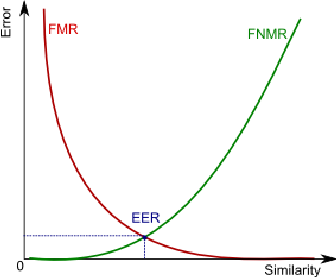
\includegraphics[width=0.5\textwidth]{assets/fnmr-fmr-eer}
	\centering
	\caption{FNMR vs FMR vs EER}
	\figuresource{A Comparison Framework for Fingerprint Recognition Methods
		(\href{https://www.researchgate.net/figure/The-Relationship-between-FNMR-FMR-and-ERR_fig3_259558386}{researchgate.net})
	}
\end{figure}

Die Equal-Error-Rate beschreibt den Schnittpunkt der beiden Fehlerraten (Falscherkennungs-Rate (FMR) und Falschablehnungs-
Rate (FNMR)). Die Schwellwert-Linie für Authentifizierungs-Entscheidungen kann nun von den Systemherstellern selbst
festgelegt werden: typischerweise sollte diese in der unmittelbaren Nähe zum EER-Punkt liegen.

Wird die Schwellwert-Linie (in der Abb. 3) rechts von der EER angesetzt wird das System zwar insgesamt sicherer (ie. die
Falscherkennungen nehmen ab), aber gleichermaßen benutzerunfreundlicher, da authentische Nutzer (häufiger) 
fälschlicherweise Abgelehnt werden und u.U. mehrere Authentifizierungsversuche vornehmen müssen um erfolgreich
erkannt zu werden.

Wird die Schwellwert-Linie (in der Abb. 3) links von der EER angesetzt, kommt es zu einem permissiven System, in dem
Nutzer im Zweifel erfolgreich authentifiziert werden. Somit wird das Gesamtsystem unsicherer, da ein Angriff hier deutlich 
einfacher ist.

Die Entscheidung wo die Schwellwert-Linie einzuzeichnen ist, ist davon abhängig zu machen in welchem Kontext das System
verwendet werden soll. Ist das biometrische System nur einer von vielen Faktoren zur Authentifizierung, oder wird in einem
zeitkritischen oder lebensbedrohlichen Szenario verwendet, kann es entgegen der Sicherheit des Systems dennoch sinnvoll 
sein, ein permissives biometrisches System zu verwenden, da die Folgen einer falschen Ablehnung (beispielsweise während 
einer Not-Operation) dramatisch sein könnten. Wird das System allerdings weder in einem zeitkritischem noch anderweitig
bedrohlichem Szenario verwendet, sollte in der Regel der Fokus auf die Sicherheit des Systems gelegt werden, was für 
einen, tendenziell, restriktiveren Ansatz des Schwellwertes spricht.


\subsection{Diagramm Zusatzaufgabe}

\annotation{
    Betrachten Sie nun nochmal das Diagramm, welches Sie für Teil b) erstellt haben.
    Nehmen Sie nun an, dass der hier eingezeichnete Graph für die FMR ausschließlich
    auf Basis anderer legitimer Nutzer („nicht-Imposter“) erstellt wurde.\\\\
    Wie würde sich im Vergleich dazu ein zweiter FMR-Graph aussehen, der die
    False-Matches von gezielten Angriffen (Impostern) wiedergibt, unter der Annahme,
    dass diese bezüglich der Merkmale der angegriffenen Personen diesen ähnlicher
    sind? Zeichnen Sie einen exemplarischen zweiten Graphen ein und erläutern Sie!\\\\
    Hinweis: überlegen Sie ggf. auch nochmal vor dem Hintergrund ihrer Lösung zu Aufgabe 3g!
}


\begin{figure}[ht]
	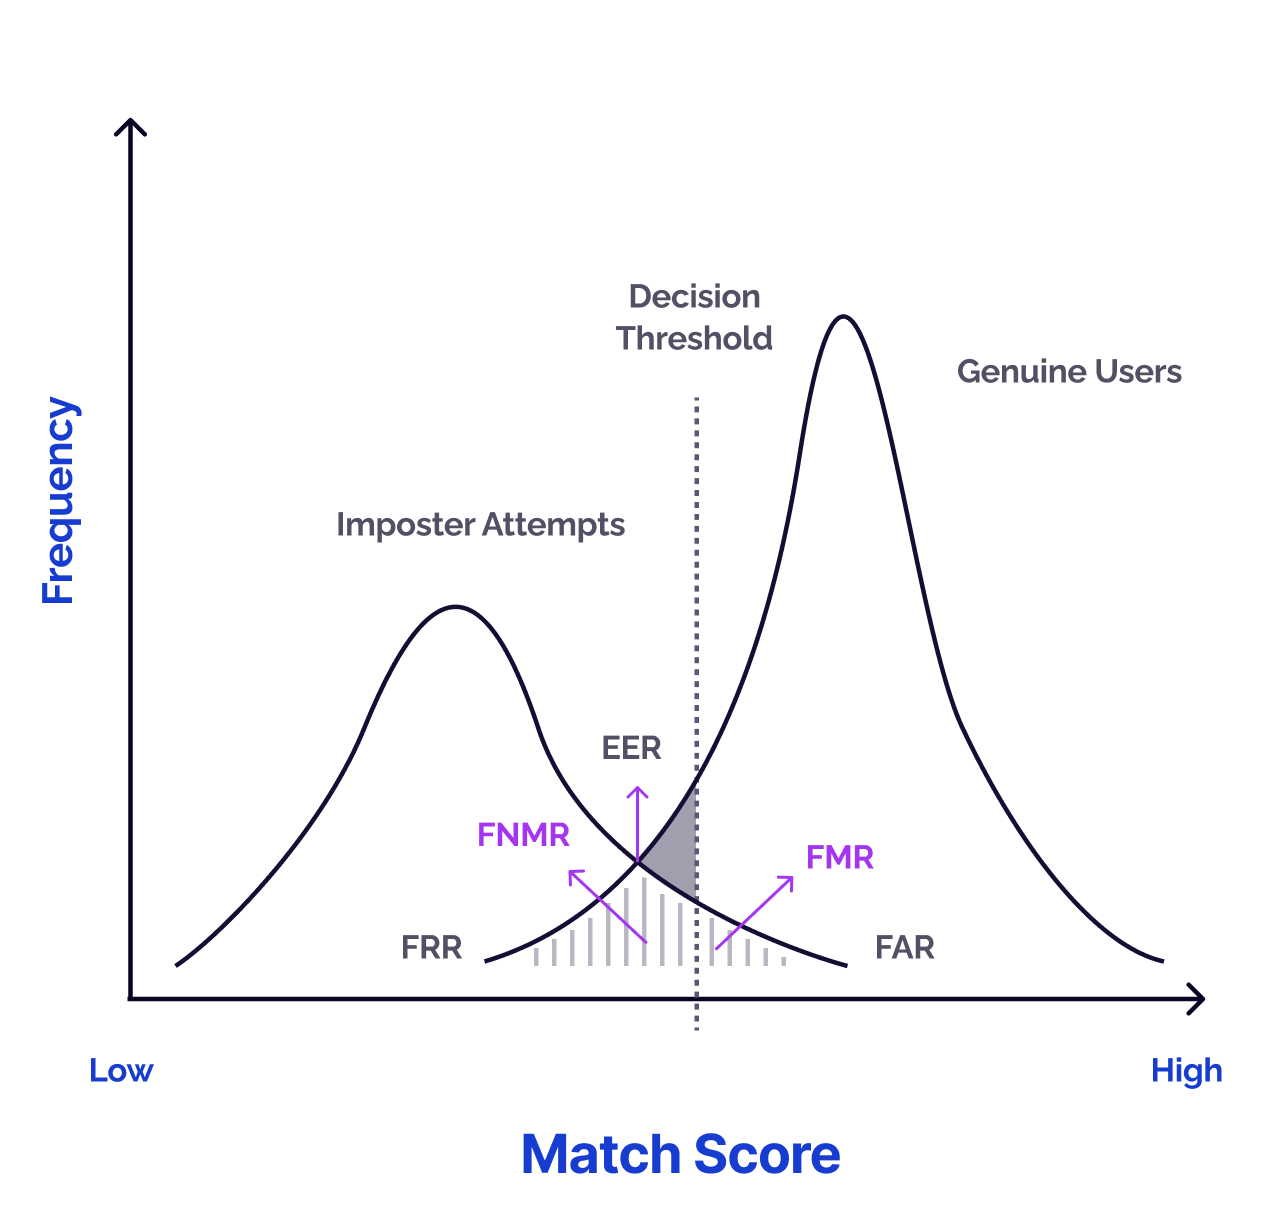
\includegraphics[width=0.5\textwidth]{assets/fnmr-fmr-eer-imposter}
	\centering
	\caption{FNMR vs FMR vs EER – Imposter}
	\figuresource{Facia AI - Knowledgebase
		(\href{https://facia.ai/knowledgebase/knowing-the-equal-error-rate-eer-in-biometrics/}{facia.ai})
	}
\end{figure}

In der hier dargestellten Grafik (Abb. 4) werden die Authentifizierungsversuche (inkl. implizierter Häufigkeit)
in einer Übersichtsgrafik dargestellt:

Der Grafik liegt im Sinne der Veranschaulichung des Sachverhaltes, die Annahme zu Grunde, dass Imposter-Versuche
tendenziell einen niedrigeren Match-Score (in Abb. 3 als ``Similarity'' beschrieben) erzielen.

Die Überschneidung von Imposter-Versuchen und Authentischen-Versuchen wird hier als EER eingezeichnet, da dieser,
genau den, in der vorherigen Aufgabe beschriebenen Scheidepunkt abbildet: Liegt die Schwellwert-Linie links, wird das 
System permissiv und somit anfällig für Imposter – liegt sie rechts vom EER wird das System restriktiv und somit sicherer,
aber gleichzeitig benutzerunfreundlicher.

Die Verbindung zwischen dieser Grafik und der Aufgabe 3g) ist ebenfalls offensichtlich erkennbar, da sich der Median-
Match-Score über alle Versuche Versuche hinweg deutlich nach unten verschiebt (angenommen, die Imposter-Versuche schneiden 
wie im o.g. Beispiel deutlich schlechter ab).

\newpage

\subsection{Statistische Signifikanz nach Doddington}

\annotation{Erklären Sie folgende Faustregeln:}

\subsubsection{Doddington’s Rule of 30}

Die Doddington's Rule of 30 wird folgendermaßen im Skript (Kapitel 4.2) eingeführt:\\[0.1em]

\textit{``Man teste, bis man insgesamt 30 Fehler erhält. Dann kann man mit 90\%iger Sicherheit annehmen, 
dass die beobachtete Fehlerwahrscheinlichkeit (z.B. FMR) innerhalb von +/- 30\% des wahren
Wertes liegt''}\\[0.1em]

Doddington's Rule of 30 bezieht sich auf die statistische Verteilung der tatsächlichen Fehlerrate durch 
Stichprobentests. Wie im Skript bezogen ist das Testen von biometrischen System nicht trivial auf Grund 
der physikalischen Abhängigkeiten der Eingabedaten. Somit lässt sich mittels Doddington's Rule of 30 auf
der Basis von Stichprobentests eine realtiv genaue (ie. laut der Regel ca. 90\%) Vorhersage über die FMR 
treffen.

\subsubsection{Doddington’s Rule of 3}

Die Doddington's Rule of 3 wird folgendermaßen im Skript (Kapitel 4.2) eingeführt:\\[0.1em]

\textit{``Wenn keine Fehler in N unabhängigen Tests auftreten, kann man mit
95\%iger Sicherheit davon ausgehen, dass die Fehlerwahrscheinlichkeit <3/N ist''}\\[0.1em]

Mittels Doddington's Rule of 3 lässt sich die FMR eines biometrischen Systems ableiten, die keine Fehler
in Stichprobentests erzielt haben. Dies ist sehr nützlich, da akkurate biometrische Tests Zeit- und 
Kosten-intensiv sind.

\subsubsection{Wie viele fehlerfreie Versuche sind nach Doddington’s Rule of 3 notwendig, um für ein biometrisches Iris-Erkennungssystem, welches während des Tests keine False-Matches generiert, mit einer 95\% Konfidenz abzuschätzen, dass es eine FMR von maximal 0,06\% hat?
}

Die Anwendung von Doddington's Rule of 3 ist trivial möglich, da lediglich die Gleichung ${3 \over N} = 0.006$ gelöst 
werden muss:

\begin{align*}
         {3 \over N} & = 0.006 \\
                   3 & = 0.006 * N \\
     {3 \over 0.006} & = N\\
     {3 \over 0.006} & = 500\\
                   N & = 500
\end{align*}

Somit lässt sich nun mit 95\%er Wahrscheinlichkeit sagen, dass die FMR des Iris-Erkennungssystems < als 0.06\% ist.

\subsubsection{Erläutern die folgende Aussage aus dem Lernmodul, finden Sie ggf. einige Beispiele, welche die Aussage begründen: „Daraus folgt: die Beobachtung von 3 Fehler in 100 Versuchen entspricht nicht automatisch der Einschätzung, dass jede der 100 Personen mit einer Fehlerquote von jeweils exakt 3\% hat!“
}

Die Aussage verweist auf die Tatsache, dass eine beobachtete Fehleranzahl in einer Stichprobe nicht direkt auf die 
individuelle Fehlerquote jedes einzelnen Testobjektes schließen lässt. Die Gründe hierfür sind:
 
\begin{enumerate}
 	\item Statistische Verteilung von Merkmalen – Unterschiedliche Testobjekte haben unterschiedliche biometrische Merkmale. Die Beobachtung von 3 Fehlern in 100 Versuchen lässt lediglich Aussagen über die Gesamtheit des Systems zu, nicht aber über einzelne Testobjekte. So kann beispielsweise ein Testobjekt das ein Merkmal mit einer hohen Trennschärfe besitzt zuverlässiger Identifiziert werden (ie. hat eine geringere Fehlerquote) als ein Testobjekt das lediglich Merkmale mit geringer Trennschärfe hat.
 	\item Stichprobenstreuung – Die Verteilung der getesteten Testobjekte in der Gesamt-Variabilität der Merkmale (Inter-Personen-Variabilität) wird nicht angegeben. Es ist gut möglich, dass die Stichproben nicht repräsentativ für die Gesamtverteilung der Merkmale ist und somit der Test in einer anderen Fehlerquote resultiert als dies im tatsächlichen Einsatz der Fall wäre.
\end{enumerate}
 
\newpage
 
\section{}

\subsection{Modalität Fingerabdruck}

\subsubsection{Benennen Sie die drei unterschiedlichen Stufen (engl. Levels) von Fingerabdruckmerkmalen}

Das Skript (5.1.1) führt die Modalität Fingerabdruck mit drei unterschiedlichen Stufen ein:

\begin{enumerate}
	\item Globale Merkmale – die Klassifizierung von zusammengesetzten Mustern der Fingerkuppe
	\item Minutien-basierte Merkmale – die Eigenschaften von einem oder mehreren Graten auf der Fingerkuppe
	\item Schweißporen-basierte Merkmale – die Klassifizierung von Poren-Mustern
\end{enumerate}

\subsubsection{Erklären Sie die Merkmalsart ``Minutien'' und skizzieren Sie 5 unterschiedliche Beispiele}

Minutien-basierte Merkmale beziehen sich auf die Eigenschaften von Graten (im einzelnen oder reziprok). Im Skript 
angeführte Beispiele sind:

\begin{itemize}
	\item Die Aufteilung eines Grates in zwei
	\item Die Terminierung eines Grates an einem Punkt
	\item Die Kreuzung von zwei oder mehreren Graten
	\item Ein unabhängiger, freistehender Grat
	\item Ein umschlossenes Tal von zwei oder mehreren Graten 
\end{itemize}

\subsection{Modalität Stimme}

\subsubsection{Benennen Sie die drei grundsätzlichen Ziele der sprachbasierten Biometrie}

Das Skript (5.2.1) führt die Modalität Stimme mit drei unterschiedlichen Zielen ein:

\begin{enumerate}
	\item Automatischen Sprechererkennung – Identität / Authentifizierung anhand des Stimm-Merkmals
	\item Textuelle Spracherkennung – Gesprochene Inhalte in einen digitalen Text zu überführen
	\item Emotionen aus Stimmcharakteristika – Identifikation von subtilen Merkmalen der Stimme / des Sprechers
\end{enumerate}

\subsubsection{Erklären Sie stichpunktartig das Konzept der ``Mel-Frequency Cepstral Coefficients (MFCC)''}

\begin{itemize}
	\item Ein Mel-Frequency-Cepstrum (MFC) beschreibt das energie Spektrum eines Geräusches
	\item Ein MFC setzt sich aus vielen Koeffizienten (MFCCs) zusammen
	\item Die MFCCs eines Geräusches lassen sich (stark vereinfacht) mittels einer kombination aus Fourier-Transformation, Überführung in die Mel-Scale, der Anwendung der Logarithmus-Funktion und einer diskreten Cosinus-Transformation ableiten.
	\item Der Unterschied zwischen einem Cepstrum und dem Mel-Frequency-Cepstrum ist die verwendung der Mel-Scale für die Aufzeichnung der Energie-Werte
\end{itemize}

\subsection{Modalität Gangart}
\annotation{Lesen Sie ggf. in der Quelle \href{http://persci.mit.edu/pub_pdfs/niyogi_XYT.pdf}{[NiAd1994]} nach.}

\subsubsection{Erklären Sie kurz das Aufzeichnungsszenario für den ``kanonischen Gang'' (``canonical walk'')}

Das Szenario für die Aufzeichnung eines kanonischen Gangs setzt voraus, dass die Kamera die das Individuum aufzeichnet im
90-Grad-Winkel zur Laufrichtung und ungefähr auf der gleichen Höhe wie die Kröpermitte platziert wird (ie. keine Top-Down 
Perspektive).

\subsubsection{Erklären Sie: welche Bildverarbeitungsschritte sind notwendig, um hieraus ein so genanntes XT Diagramm zu generieren}

\begin{enumerate}
	\item Entfernung von Hintergrundinformationen
	\item Kantenerkennung
	\item Extraktion der XT-Schnittlinie
	\item Pixel-Extraktion entlang der Linie
	\item Aufbau des XT-Diagramms
\end{enumerate}

\subsubsection{Überlegen, recherchieren und beschreiben Sie 5 Merkmale, welche aus XYT Diagrammen gewonnen werden können}

Die folgenden 5 Merkmale bzw. Prozessierungsschritte können aus einem XYT Diagramm extrahiert werden bzw. darauf 
ausgeführt werden.

\begin{enumerate}
	\item Geschwindigkeit und Beschleunigung
	\item Trajektorienanalyse
	\item Periodizität und Frequenzanalyse
	\item Interaktionsanalyse
	\item Anomalieerkennung
\end{enumerate}

\subsection{Modalität Tastaturanschlag}

\subsubsection{Benennen Sie Vorteile und Anwendungen dieser biometrischen Modalität}

Die Modalität der Tastaturanschläge bietet weitreichende Vorteile hinsichtlich ihres möglichen Einsatzgebietes, da:

\begin{enumerate}
	\item Keine Sensor-Notwendigkeit – Tastaturanschläge lassen sich mit jedem (tastatur-basiertem) Eingabegerät aufzeichnen ohne besondere Hardware
	\item Gute Performance in textabhängigen Tests – Tastaturanschläge sind in Szenarien in denen die Eingabedaten bekannt sind sehr aussagekräftig über die Identität
\end{enumerate}

Das Tastaturanschlagsmuster kann z.B. als weiteren Faktor bei der Passwort-Authentifizierung verwendet werden, um zu 
erkennen, wenn ein Imposter versucht sich in dem System anzumelden.

\subsubsection{Erläutern Sie kurz das Konzept der ``Digraph'' und überlegen und beschreiben Sie die vier Merkmale, die aus einem Digraph gemessen werden können}

Ein ``Diagraph'' ist das Segment von 2 aufeinanderfolgenden Tastenanschlägen.
Vier Merkmale die anhand von Diagraphen einer Eingabe abgeleitet werden können sind:

\begin{enumerate}
	\item Inneres Delta – die Zeit zwischen den Tasten innerhalb eines Diagraphen
	\item Äußeres Delta – die Zeit zwischen zwei Diagraphen
	\item Repetitions-Interval – Wie häufig ein Diagraph verwendet wird
	\item Dauer – Wie lange ein Diagraph (von keydown der ersten Taste zu keyup der zweiten) dauert
\end{enumerate}

\subsubsection{Argumentieren Sie mathematisch/logisch, wie das biometrische Verfahren Tastaturanschlag zur Verbesserung der Passwortsicherheit eingesetzt werden kann und stellen Sie klar, welche Annahmen Sie dabei tätigen}

Wie bereits unter 1) angeführt könnte die Tastaturanschlags-Modalität als zusätzlicher Faktor bei der 
Passwort-Authentifizierung dienen. Hierbei kann das System das Eingabemuster des Authentischen-Benutzers lernen und
verwenden, um (bei einer starken Abweichung) einen Imposter zu erkennen, obwohl das Passwort korrekt eingegeben wurde.

Somit wird das System resilient(er) gegenüber Passwortdiebstahl – es könnte z.B. bei einer starken Abweichung das 
Passwort zurücksetzen. Die Tastaturanschlags-Modalität eignet sich, wie im Skript angeführt, sehr gut für diesen
Anwendungsfall, da der Eingabetext bekannt ist.

\subsection{Modalität Handschrift}

\subsubsection{Benennen Sie die beiden grundlegenden Kategorien von Merkmalen handschriftbasierter Biometrie}

Die beiden grundlegenden Kategorien von Merkmalen handschriftbasierter Biometrie sind:

\begin{itemize}
	\item Statische Merkmale: Alle Merkmale, die aus einem statischen Bild der Handschrift extrahiert werden können (z. B. eingescannter Zettel).
	\item Dynamische Merkmale: Alle Merkmale, die während des Schreibprozesses erfasst werden und Bewegungsabläufe sowie zeitliche Eigenschaften beschreiben.
\end{itemize}

\subsubsection{Welche Arten von Signalen können durch Handschrift-Digitalisiertabletts erfasst und aufgezeichnet werden, beschreiben Sie}

\begin{enumerate}
	\item Position der Hand
	\item Position des Stifts (z.B. Koordinaten)
	\item Druck
	\item Stift-Berührungen des Displays
	\item Neigung
	\item Zeitstempel
\end{enumerate}

\subsubsection{Benennen Sie 5 Beispiele von statistischen Merkmalen, die aus Handschrift-Signalen zur biometrischen Erkennung berechnet werden können}

\begin{enumerate}
	\item Strichlänge
	\item Frequenz der Stift-Berührungen
	\item Schreibwinkel
	\item Schleifen
\end{enumerate}

\subsubsection{Benennen Sie 4 alternative Semantikklassen zur Unterschrift und diskutieren Sie deren Vor- und Nachteile}

\begin{enumerate}
	\item Wörter
	\item Sätze
	\item Zahlen
	\item Freitext
\end{enumerate}

\subsection{Überlegen und benennen Sie jeweils mindestens einen möglichen Sensortyp für die folgenden Modalitäten:}

\begin{itemize}
	\item Handschrift – optischer Sensor
	\item Fingerabdruck – optischer Sensor
	\item Sprache – Mikrofon
	\item Gesicht – optischer Sensor, LIDAR
	\item Iris – optischer Sensor
	\item Finger-/Handgeometrie – optischer Sensor, LIDAR
	\item Gangerkennung – optischer Sensor
	\item DNA – N/A
\end{itemize}

\subsection{Führen Sie die praktische Übung „Handgeometrie“ durch!}
\subsection{Führen Sie die praktische Übung „Offline Handschrift“ durch!}

\end{document}
